% !TeX root = main.tex

\section{Approche}

	Dans cette partie, nous expliquerons quels sont les différents outils et stratégies mis en place pour permettre la résolution du problème.
	
	La principale difficulté c'est que le jeu de base est trop complexe et ne permet pas de déterminer si l'approche actuelle est mieux adapté. Par conséquent, on utilisera des instances plus petites, qui sont des plateaux de plus petite taille ($4\times 4, 5\times 5, \dots$) qui respectent les deux lois d'Eternity II. 
	
	En supposant que la smartforce devient de plus en plus bénéfique suivant la complexité du problème, il est nécessaire de mettre en place une valeur étalon, reposant sur un programme bruteforce qui fournit différentes données permettant d'estimer si cette supposition est vraie.
	
	Chaque n\oe ud de l'arbre des possibilités du jeu doit satisfaire deux données :
	
	\begin{description}
		\item[variable] : une des cases
		\item[valeur] : une des pièces.
	\end{description}
	
	Lors de la progression dans l'arbre, il faut définir quelle valeur sera définie pour quelle variable (choisir telle case sur laquelle sera placée telle pièce). Pour cela, chaque variable (case) possède un domaine de valeur, un tableau contenant contient toutes les valeurs possibles (toutes les pièces qui peuvent être mise dessus) que l'on appellera \textbf{domaine}.
	
	Et inversement, chaque valeur (pièce) possède un domaine contenant toutes les variable à laquelle elle peux être appliquée.
	
	Il est possible de déterminer théoriquement, suivant l'instance actuelle, la taille du domaine pour chaque pièce ou case. En effet, en connaissant la moyenne de distribution des couleurs par pièces, il est possible d'évaluer la quantité de pièces à chaque case ou la quantité de pièces adjacentes à une autre pièce.
	
	\begin{exmp}
		Pour un plateau de taille 4. La case en position $(O,O)$ à 4 pièces posables, La distribution des couleurs de ces pièces est equitable (voir \autoref{fig:4_pieces_on_bordure}), par conséquent, elles possèdent toutes les couleurs possibles pour les pièces de bord. Par conséquent, si l'on ne définit pas la pièce qui est placé sur la case en $(0,0)$, jusqu'à 8 pièces peuvent être placés en $(0,1)$ et $(1,0)$.
	\end{exmp}
	\begin{rem}
		 Dans la pratique, chaque couleur n'à pas la même quantité de pièces. Par conséquent, ce résultat peux varier. Mais il permet d'évaluer le plafond supérieur du nombre de cas possible pour une corolle ou le nombre de cas possibles total.
	\end{rem}
\newpage

	\subsection{Bruteforce}
	
	Le programme de bruteforce nous fournit une valeur étalon. Il se contente de parcourir tout l'arbre des possibilités.
	
	Il permet aussi de savoir quelle stratégie de parcours du plateau est la plus bénéfique. Les différentes stratégies de choix de variable étalonnées sont :
	
	\begin{figure}[H]
		\minipage{0.32\textwidth}
		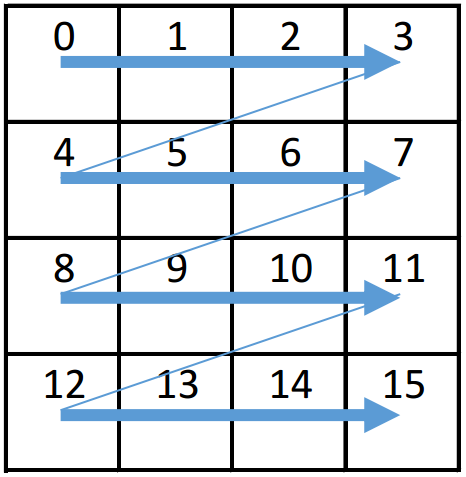
\includegraphics[width=\linewidth]{images/parcours_rowscan.png}
		\caption{\textbf{rowscan} : parcours horizontal du plateau}\label{fig:parcours_rowscan}
		\endminipage\hfill
		\minipage{0.32\textwidth}
		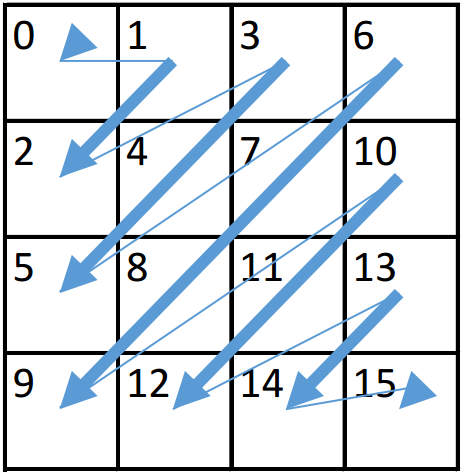
\includegraphics[width=\linewidth]{images/parcours_diagonal.png}
		\caption{\textbf{diagonal} : parcours diagonal du plateau}\label{fig:parcours_diagonal}
		\endminipage\hfill
		\minipage{0.32\textwidth}
		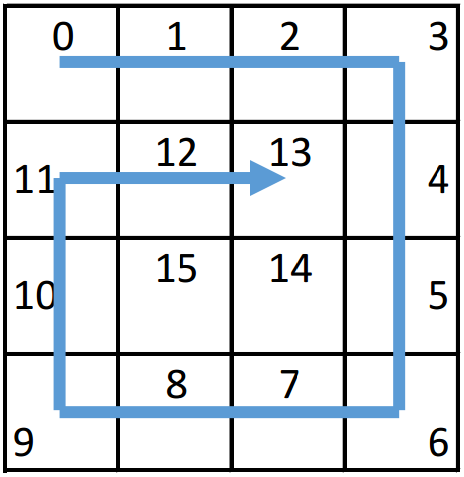
\includegraphics[width=\linewidth]{images/parcours_spiral-in.png}
		\caption{\textbf{spiral-in} : parcours en spirale fermente du plateau}\label{fig:parcours_spiral-in}
		\endminipage\hfill
	\end{figure}
	\begin{figure}[H]
		\minipage{0.32\textwidth}
		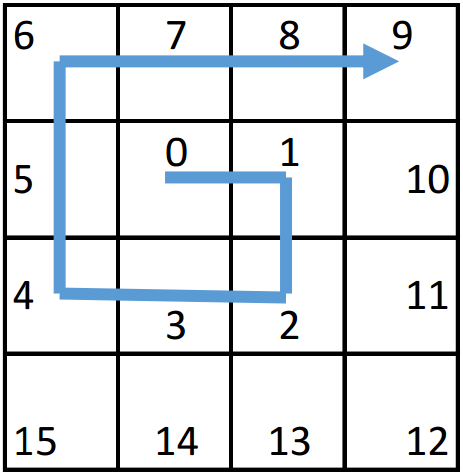
\includegraphics[width=\linewidth]{images/parcours_spiral-out.png}
		\caption{\textbf{diagonal} : parcours en spirale ouvrante du plateau}\label{fig:parcours_spiral-out}
		\endminipage\hfill
		\minipage{0.32\textwidth}
		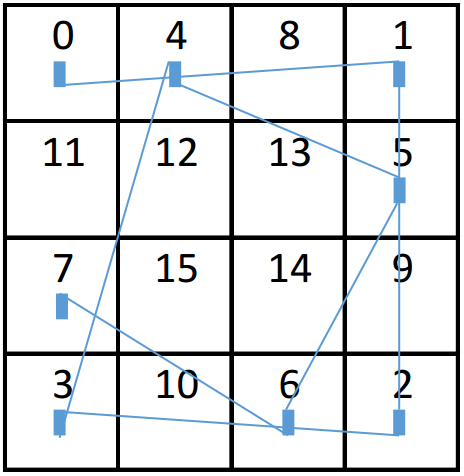
\includegraphics[width=\linewidth]{images/parcours_quad-spiral-in.png}
		\caption{\textbf{quad spiral out} : parcours avec quatre spirales fermentes}\label{fig:quad-spiral-in}
		\endminipage\hfill
		\minipage{0.32\textwidth}
		\ %don't touch this !
		\endminipage\hfill
	\end{figure}
	
	Le choix des pièces (valeurs) est fait dans l'ordre lexicographique (ordre par défaut).
	
	Les données utilisés pour l'étalonnage sont les suivants :
	
	\begin{description}
		\item[Première solution] : le temps et la quantité de n\oe uds nécessaires pour trouver la première solution (chaque instance peux en avoir plusieurs)
		\item[Nombre total de solutions] : pour estimer les placement des solutions dans l'arbre
		\item[Nombre total de n\oe uds] : pour pouvoir estimer la rapidité de l'algorithme pour trouver la première solution
		\item[Temps total] : pour connaître si l'algorithme utilisé est plus performant que celui d'avant
	\end{description}
\newpage

	\subsection{Smartforce}

	Le principe de la smartforce repose sur la quantité de données qu'elle possède. Par conséquent, il est important que ces données soient bien organisées afin de pouvoir les traiter avec aise. Ces données sont organisées pour former des modèles. Chaque modèle peut être interprété comme un point de vue différent du problème. La liaison de plusieurs modèles variés fait la puissance de la smartforce.
	
	On note aussi l'introduction de nouvelles méthodes de parcours :
	
	\begin{itemize}
		\item Choix de variable :
		\begin{itemize}
			\item\textbf{Optimiste} : on choisit la variable qui à le plus grand domaine
			\item\textbf{Pessimiste} : on choisit la variable qui à le plus petit domaine
		\end{itemize}
		\item Choix de valeur :
		\begin{itemize}
			\item \textbf{Lexicographique} : utilisé par défaut par la bruteforce, on choisit la valeur suivante dans l'ordre par défaut.
			\item \textbf{Optimiste} : la valeur dont le domaine est le plus grand.
			\item \textbf{Pessimiste} : la valeur dont le domaine est le plus petit.
		\end{itemize}
	\end{itemize}
	
	Différents modèles seront donc présentés par ordre de difficulté, car, afin de fournir des types de données variés, il est nécessaire d'abstraire le problème initial.

	\subsubsection{CaPi}

	CaPi est le plus simple modèle représentant le problème. Il a pour variable les cases (identifiées par un numéro ou par ses coordonnées sur le plateau) et pour valeur les pièces (identifiées par un numéro et par leur rotation). C'est aussi lui qui est utilisé comme modèle par défaut pour le choix des valeurs et variables.
	
	En somme, chaque pièce est associé aux cases sur laquelle elle peut être posée et inversement, chaque case contient la liste des pièces qu'elle peux avoir.
	
	\begin{rem}
		Le domaine des cases est un peu plus complexe : une pièce donnée peux être placée sur la case \enquote{jusqu'à 4 fois} (à plusieurs rotation différentes). Par conséquent, lorsque l'on met à jour le domaine de la case (en posant la pièce sur une autre case), on supprime toutes les occurrences de cette pièce du domaine en question.
		
		Par conséquent, chaque pièce possède en vérité quatre domaines distincts (correspondant à chaque rotation de la pièce).
	\end{rem}
\newpage

	\subsubsection{BoCo}
	
	Le modèle BoCo (Bordures/Couleurs) est une approche bien plus fine, elle découle de l'abstraction de CaPi.
	
	Si l'on connait le domaine d'une case. On connaît les pièces qui peuvent être posés dessus. Par conséquent, on définit une \textbf{Bordure} comme une sous-partie d'une case.
	
	\begin{exmp}
		Prenons la case 0, en $(0,0)$ sur le plateau. Elle peux contenir 4 pièces (\no 0,1,2,3 ; ce sont toutes des pièces de coin) en la rotation 0.
		
		\minipage[t]{0.29\textwidth}
		Si l'on décompose la case, celle-ci contient 4 faces :
		
		\begin{figure}[H]
			\includestandalone[width=\linewidth]{graphics/case}

			\caption{Détails d'une case}\label{fig:case}
		\end{figure}
		
		Les bords 1 et 2 étant gris, il n'est pas nécessaire de les représenter. 
		\endminipage\hfill
		\minipage[t]{0.29\textwidth}
	
		On décompose ensuite les 4 pièces :
		\begin{figure}[H]
			\includestandalone[width=\linewidth]{graphics/4_pieces}
			\caption{Couleurs des 4 pièces}\label{fig:4_pieces}
		\end{figure}
		\endminipage\hfill
		\minipage[t]{0.29\textwidth}
			On associe ensuite les couleurs et leur occurence à chaque bord :
			\begin{figure}[H]
				\includestandalone[width=\linewidth]{graphics/4_pieces_on_bordure}
				
				\caption{Occurrences et couleurs de bordures}\label{fig:4_pieces_on_bordure}
			\end{figure}
		\endminipage\hfill
	\end{exmp}
	
	Cette simplification du problème nous permet de connaître plus simplement si deux cases adjacentes possèdent des matching non possibles.  Il suffit ensuite d'éliminer les pièces possèdent la couleur manquante.
		
	\begin{exmp} Dans cet exemple, pour le deuxième cas [\autoref{fig:bordure_no_match}], toutes les pièces (orientées) ayant du rouge sur la face 2 ne peuvent être posées sur la case. Cela vaut aussi pour la case adjacente où la couleur verte ne peux être posée.
			
		\minipage[t]{0.45\textwidth}
			Les deux cases ont des matching possibles :
			
			\begin{figure}[H]
				\includestandalone[width=\linewidth]{graphics/bordure_match}
				\caption{Cases adjacentes avec matching possible}\label{fig:bordure_match}
			\end{figure}
		
		\endminipage\hfill
		\minipage[t]{0.45\textwidth}
			Les deux cases ont des matching non possibles
			
			\begin{figure}[H]
				\includestandalone[width=\linewidth]{graphics/bordure_no_match}
				\caption{Cases ayant des matching non possibles}\label{fig:bordure_no_match}
			\end{figure}
			\endminipage\hfill
	\end{exmp}
	
	Les bordures sont identifiées par un numéro. Chaque \textbf{bordure} possède un domaine contenant les \textbf{couleurs} uniques qu'elle peux avoir et leur cardinalité [\autoref{fig:4_pieces_on_bordure}].
	
	Les couleurs sont aussi identifiés par un numéro. Chaque \textbf{couleur} contient l'ensemble des bordures où elle peux être placée, et combien de fois elle peux l'être (cardinalité).
	
	L'utilité de ce modèle réside dans la propagation des données. Le but étant de propager une information à travers les cases, en ne mettant à jour que les données concernées.
	
	Dans une disposition CaPi, pour appliquer la propagation des données, on est obligé de faire le produit des domaines des cases adjacentes pour chaque matching (comparer les pièces possibles de chaque case entre eux). Ce qui s'avère très couteux et beaucoup de ces vérifications sont inutiles.
	
	Par contre, grâce à \textbf{BoCo}, il suffit de vérifier que la cardinalité des couleurs reste positive pour les deux bordures adjacentes. Seulement lorsque le nombre d'occurrences d'une couleur tombe à zéro, l'autre est invalidée (disons, la couleur rouge). Il suffit ensuite de récupérer les autres couleurs de la pièce qui disparait (car elle avait la couleur rouge), et de décrémenter les autres bordures de la case concernée. Si leur occurrence tombe à zéro, on met à jour leur bordure adjacente, sinon, la propagation s'arrête.

	\begin{exmp}
		Si une couleur disparait, alors toutes les pièces l'ayant ne peuvent plus être placées à cette case, par conséquent, les autres bords de la case ont (probablement) des couleurs qui disparaissent aussi (propagation de la disparition).
	\end{exmp}

	\subsubsection{Corolles}


	Une corolle est une surface du plateau qui est pré-calculée afin de pouvoir être réutilisée par la suite.
		
	La corolle possède une pièce centrale, de laquelle sont calculées les pièces avoisinantes. Par conséquent, la taille de la corolle est définie par la distance de la pièce la plus au bord par rapport à la pièce centrale, cette distance sera appelée hamming ($H$).
	
	\begin{rem}
		Une corolle de hamming 0 est la pièce elle-même.
	\end{rem}
		
	\begin{figure}[H]
		\begin{minipage}[t]{0.33\textwidth}
			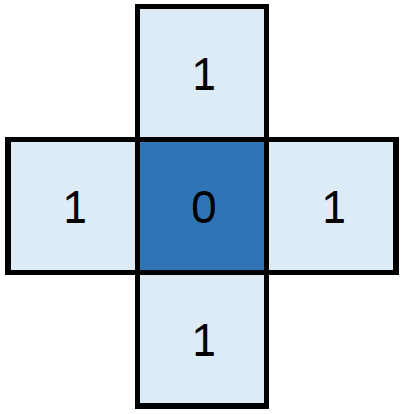
\includegraphics[width=\linewidth]{images/corolle_hamming_1.png}
			\caption{Corolle de hamming 1}\label{fig:corolle_hamming_1}
		\end{minipage}\hfill
		\begin{minipage}[t]{0.33\textwidth}
			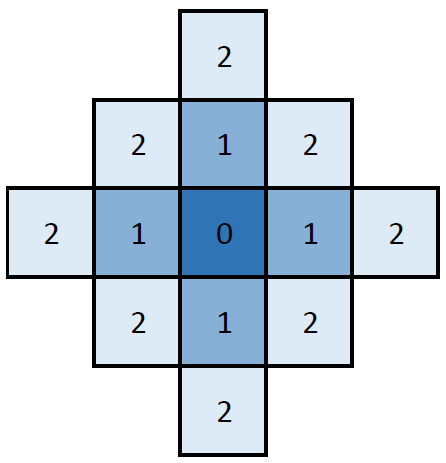
\includegraphics[width=\linewidth]{images/corolle_hamming_2.png}
			\caption{Corolle de hamming 2}\label{fig:corolle_hamming_2}
		\end{minipage}\hfill
		\begin{minipage}[t]{0.33\textwidth}
			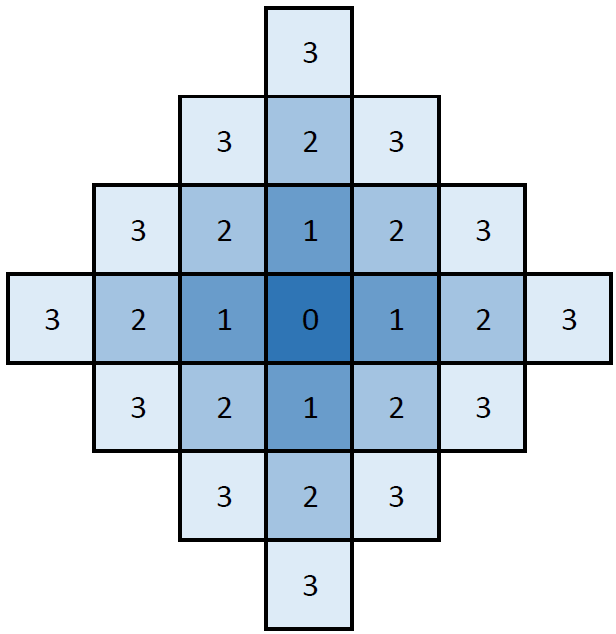
\includegraphics[width=\linewidth]{images/corolle_hamming_3.png}
			\caption{Corolle de hamming 3}\label{fig:corolle_hamming_3}
		\end{minipage}\hfill
	\end{figure}

	Son nom, corolle, vient de sa forme. Suivant son placement, cette forme change. Les différentes formes dépendent de la taille de la corolle (\enquote{rayon} de la corolle) et de la position sur le plateau.
		
	\begin{figure}[H]
		\begin{minipage}[t]{0.33\textwidth}
			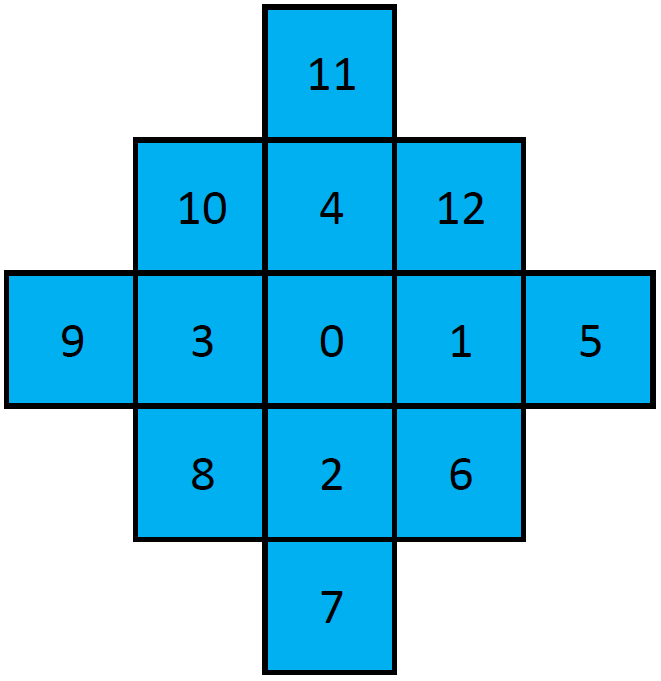
\includegraphics[width=\linewidth]{images/corolle_simple.png}
			\caption{Ordre de placement des pièces d'une corolle de Hamming 2}\label{fig:corolle}
		\end{minipage}\hfill
		\begin{minipage}[t]{0.66\textwidth}
			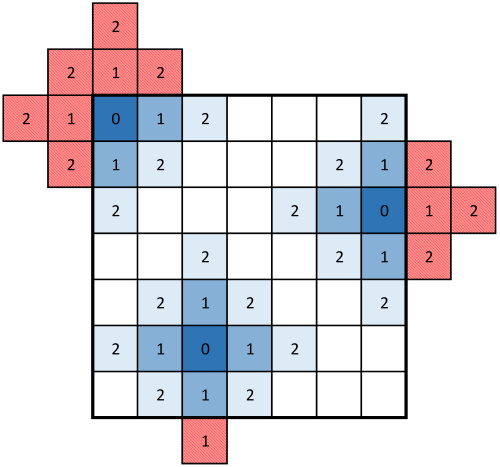
\includegraphics[width=\linewidth]{images/corolle_formes.png}
			\caption{Différentes formes de la corolle de hamming 2 sur une instance de taille 7}\label{fig:corolle_forme}
		\end{minipage}\hfill
	\end{figure}
	
	\begin{exmp}
		Supposons qu'une corolle est seulement définie par sa forme. Prenons comme coordonnées $(0,1)$ et $(1,0)$ avec un hamming de 1. La forme des corolles sur ces coordonnées est identique. Elle à une forme de tétris.
		
		Par conséquent, les corolle en coordonnées $(0,1)$ peuvent aller en $(1,0)$ et inversement.
		
		\begin{figure}[H]
			\begin{minipage}{0.33\textwidth}
				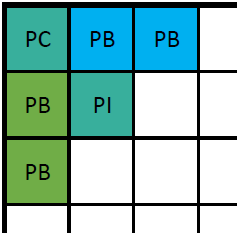
\includegraphics[width=\linewidth]{images/corolle_tetris_bord.png}
				\caption{Corolle en $(0,1)$ (blue)et en $(1,0)$ (vert)}\label{fig:corolle_tetris_bord}
			\end{minipage}\hfill
			\begin{minipage}{0.33\textwidth}
				\begin{center}
					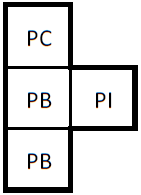
\includegraphics{images/corolle_tetris_1.png}
					\caption{Corolle tetris en $(1,0)$}\label{fig:corolle_tetris_1}
					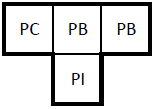
\includegraphics{images/corolle_tetris_2.png}
					\caption{Corolle tetris en $(0,1)$}\label{fig:corolle_tetris_2}
				\end{center}
			\end{minipage}\hfill
			\begin{minipage}{0.33\textwidth}
				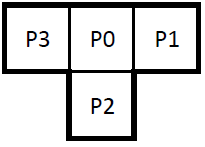
\includegraphics{images/corolle_tetris.png}
				\caption{Noms des pièces dans la corolle tetris}\label{fig:corolle_tetris}
			\end{minipage}\hfill
		\end{figure}
		
		Or, pour les types de pièces, il y a un problème. en $(1,0)$ P3 est une pièce de coin, alors qu'en $(0,1)$ c'est une pièce de bord (même problème pour P1).
		
		Donc, non seulement, une corolle est définie par sa forme, mais aussi par sa position.
	\end{exmp}
	
	Par conséquent, une corolle est définie par le type de pièces (coin, bord, intérieur) qui la composent et de sa forme. il n'est pas nécessaire de pré-calculer les corolles sur toutes les cases du plateau, il suffit de partager le plateaux en zones. Toutes les corolles d'une même zone sont identiques.
	
	\begin{rem}
		Plus le hamming de la corolle augmente, plus il y a des zones différentes à cause de l'augmentation des types de pièces qui la compose.
	\end{rem}
	
	\begin{figure}[H]
		\begin{minipage}{0.49\textwidth}
			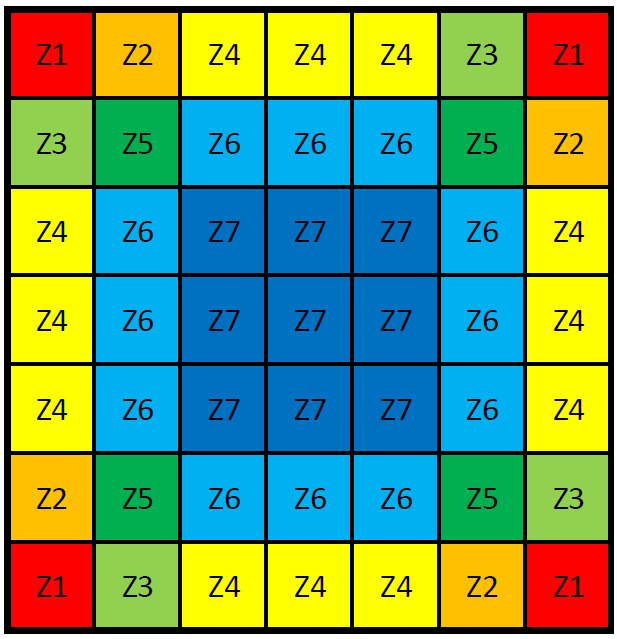
\includegraphics[width=\linewidth]{images/corolle_zones_h_1.png}
			\caption{Quantité de zones differentes sur un plateau de taille 7, pour une corolle de hamming 1}\label{fig:corolle_zones_h_1}
		\end{minipage}\hfill
		\begin{minipage}{0.49\textwidth}
			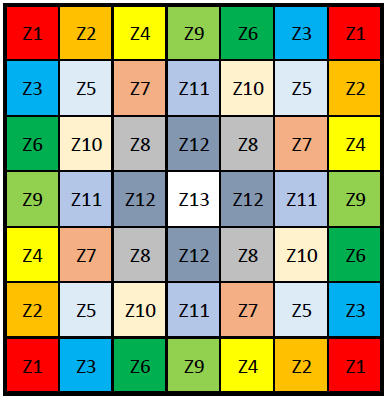
\includegraphics[width=\linewidth]{images/corolle_zones_h_2.png}
			\caption{Quantité de zones différentes sur un plateau de taille 7, pour une corolle de hamming 2}\label{fig:corolle_zones_h_2}
		\end{minipage}\hfill
	\end{figure}
	
	
	Il est possible de déterminer le nombre de zones qui composent un plateau. Elle contient 2 variables, $T$ la taille du plateau $H$ le hamming. La quantité de zones $z$ est définie par la relation suivante :
	
	\[
		\begin{cases}
		z=(H+1)^2 + H+2 &\text{si } M > H+1  \text{ avec } M\frac{T + T\%2}{2}\\
		z= \frac{T + T\%2}{2}^2&
		\end{cases}	
	\]
	
	Il y a deux cas :
	
	\begin{enumerate}
		\item Soit  $M$ la moitié (arrondie au supérieur) de la taille du plateau. Si $M> H+1$.
		
		Dans ce cas, Toutes les cases de $(0,0)$ jusqu'en $(H,H)$ sont des zones différentes (toutes ces cases sont en contact avec au moins deux bords du plateau), plus toutes les cases de $(H+1,0)$ jusqu'à $(H,H+1)$ (ceux la ne sont en contact qu'avec un seul bord) et enfin la pièce en $(H+1,H+1)$ qui ne contient que des pièces d'intérieur.
		
		\item, si le $H+1$ est supérieur ou égal, alors toutes les cases de $(0,0)$ jusqu'en $(M,M)$ sont des zones distinctes.
	\end{enumerate}
	
	
	L'espace réel dépend aussi de la taille du hamming.
	
	On a donc deux cas : 
	
	\begin{defn}
	Pour tout corolle ayant pour pièce centrale $P$ et de taille $H$ d'une zone $Z_1$ donnée, elle découle de l'expansion d'une corolle de
	taille inférieure $H-1$ ayant pour zone $Z_0$ englobant la zone $Z_1$ avec $P$ identique.
	\end{defn}
	\begin{exmp}
		Dans la ~\autoref{fig:corolle_zones_h_2}, les zones 8,12,13 sont englobées par la zone 7 de H1 [\autoref{fig:corolle_zones_h_1}].
		
		Par conséquent, toutes les corolles des zones 9,12,13 en hamming 1 sont une extension des corolles de la zone 7 en hamming 1.
	\end{exmp}

	La frontière définit les couleurs au bord de la corolle, ils sont nécessaires pour connaitre les pièces qui peuvent être placées à côté.
	
	\begin{exmp}
		Les faces d'une pièce sont la frontière d'une corolle de hamming 0.
	\end{exmp}
	
	\textbf{Rotation de la corolle}
	
	Les corolles concernées par les rotations sont les corolles qui ont au moins une pièce de bord ou de coin. Les pièces de bords et de coin ayant une orientation définie à cause de leur face grise.
	
	\begin{exmp}
		Prenons la zone Z5 de la \autoref{fig:corolle_hamming_1}, suivant l'endroit où elle se trouve, la composition de la corolle est la même, mais \enquote{tournée} : \\
		\begin{minipage}{0.24\textwidth}
			\begin{figure}[H]
				\centering
				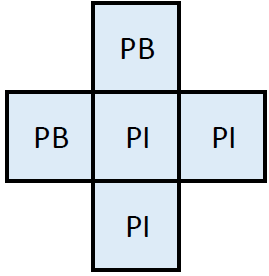
\includegraphics[width=\linewidth]{images/corolle_zone_orientee}
				\caption{Corolle de hamming 1 avec les types de pièces en $(1,1)$}
				\label{fig:corolle_zone_orientee}
			\end{figure}
		\end{minipage}\hfill
		\begin{minipage}{0.24\textwidth}
			\begin{figure}[H]
				\centering
				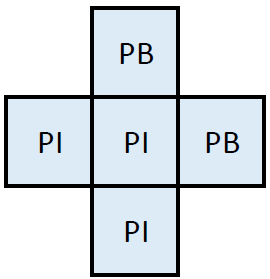
\includegraphics[width=\linewidth]{images/corolle_zone_orientee_1}
				\caption{Corolle de hamming 1 avec les types de pièces en $(5,1)$ }
				\label{fig:corolle_zone_orientee_1}
			\end{figure}
		\end{minipage}\hfill
		\begin{minipage}{0.24\textwidth}
			\begin{figure}[H]
				\centering
				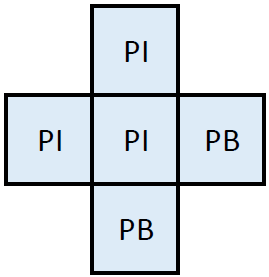
\includegraphics[width=\linewidth]{images/corolle_zone_orientee_2}
				\caption{Corolle de hamming 1 avec les types de pièces en $(5,5)$}
				\label{fig:corolle_zone_orientee_2}
			\end{figure}
		\end{minipage}\hfill
		\begin{minipage}{0.24\textwidth}
			\begin{figure}[H]
				\centering
				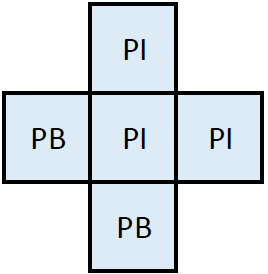
\includegraphics[width=\linewidth]{images/corolle_zone_orientee_3}
				\caption{Corolle de hamming 1 avec les types de pièces en $(1,5)$}
				\label{fig:corolle_zone_orientee_3}
			\end{figure}
		\end{minipage}\hfill
		
		La composition et la forme est la même, mais l'ordre est différent (voir \autoref{fig:corolle}).
	\end{exmp}
	
	Pour résumer. Une corolle est une surface du plateau d'une certaine forme qui est pré-calculée. Une corolle pouvant être à plusieurs endroit, elle est dépendante d'une zone. Elle est composée d'une pièce principale qui la définit ainsi que d'une frontière. Une corolle est composée d'une corolle de hamming inférieur, se trouvant dans une zone englobant la celle de la corolle actuelle. Certaines corolles d'une même zone peuvent être différents à cause de leur \enquote{rotation}.
	
	Afin que la corolle soit correcte, il est nécessaire de connaître les informations suivantes :
	\begin{itemize}
		\item taille du plateau
		\item zone de la corolle
		\item la rotation de la corolle
		\item son hamming
		\item les pièces qui la composent
	\end{itemize}
\newpage	

	\subsubsection{BoCoDiag}
	
	
	BoCoDiag est un modèle permettant de lier des couples de couleurs. Son principe est presque le même que pour BoCo, d'où le nom. La différence est que le couple est indirect.
	
	\begin{exmp}
		Prenons un zone de 4 cases.
		
		Le principe de BoCoDiag est de récupérer les liaisons diagonales. On en obtiens un couple de couleurs non identique. et pourtant, il contraint 4 couleurs.
		
		Dans cet exemple, le couple (Bleu/Blue) est lié à (Rouge/jaune) en direction Sud-Est et le couple (Blue/Jaune) est lié au couple (Bleu/Rouge). 
		
		\begin{note}
			La lecture des couleurs se fait dans le sens horaire en commencent par la face à l'ouest de la pièce.
		\end{note}
		\begin{minipage}{0.30\textwidth}
			\begin{figure}[H]
				\includestandalone[width=\linewidth]{graphics/bocodiag}
				\caption{4 pièces matchés}\label{fig:bocodiag}
			\end{figure}		
		\end{minipage}\hfill
		\begin{minipage}{0.30\textwidth}
			\begin{figure}[H]
				\includestandalone[width=\linewidth]{graphics/bocodiag_abstract_1}
				\caption{Premier couple BoCoDiag}\label{fig:bocodiag_1}
			\end{figure}		
		\end{minipage}\hfill
		\begin{minipage}{0.30\textwidth}
			\begin{figure}[H]
				\includestandalone[width=\linewidth]{graphics/bocodiag_abstract_2}
				\caption{Deuxième couple BoCoDiag}\label{fig:bocodiag_2}
			\end{figure}		
		\end{minipage}\hfill	
	\end{exmp}
	\newpage
	
	\subsection{Corolles dynamiques et marécage}
	
	La limitation principale des corolles est que l'espace pré-calculé est souvent l'ensemble des pièces possibles à ses cases. Par conséquent, le fait de traiter une donnée qui nous informe que tout est possible est inutile. D'où l'intérêt des corolles dynamiques. Les corolles dynamiques sont polymorphes et n'ont pas forcément un hamming déterminé. Elle s'agrandissent lorsque qu'une case adjacente [à la corolle dynamique] voit son domaine restraint.
	
	\begin{exmp}
		Prenons un plateau de taille 7 dans sa disposition initiale. Plaçons la corolle en $(1,2)$
		
		\begin{figure}[H]
			\centering
			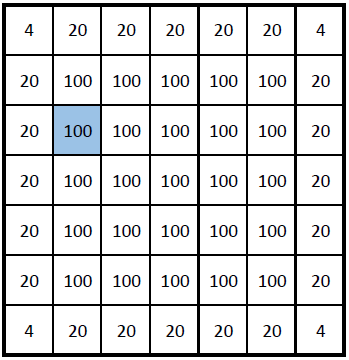
\includegraphics{images/corolle_dynamique}
			\caption[Répartition des pièces sur un plateau de taille 7]{Répartition des pièces sur un plateau de taille 7}
			\label{fig:corolle_dynamique}
		\end{figure}
		
		\begin{note}
			 Il y a 25 pièces intérieures, 4 rotation sont possibles par pièce, par conséquent, 100 \enquote{pièces} sont posables sur une case d'intérieur.
		\end{note}
		
		Dans cette figure, il n'est pas nécessaire de calculer la corolle en Hamming 1 ou plus, car ce ne sera que tout les cas possibles, on appèle donc le Hamming 1 le marécage.
		
		Placons maintenant la pièce 0 en $(0,0)$ 
		
		\begin{figure}[H]
			\centering
			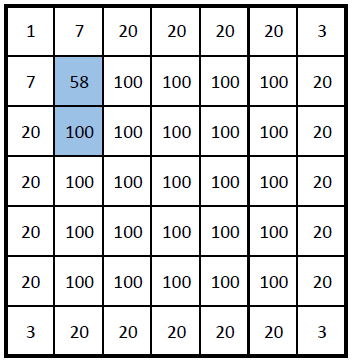
\includegraphics{images/corolle_dynamique_agrandissement}
			\caption[Répartition des pièces sur un plateau de taille 7]{Répartition des pièces sur un plateau de taille 7}
			\label{fig:corolle_dynamique_agrandissement}
		\end{figure}
		
		La case en $(1,1)$ voit son domaine réduit. Par conséquent il est malin d'agrandir la corolle vers cette case car elle pourrait nous fournir plus de données.

		\begin{note}
			Cet exemple est naïf mais illustre bien le principe de corolle dynamique et de marécage
		\end{note}
	\end{exmp}
	\newpage
	
	\subsection{Ouvertures}
	
	Grâce à l'approche Smartforce et surtout grâce au modèle \textbf{Corolle} il est possible d'initialiser efficacement les ouvertures.
	
	Pour ce faire, il suffit de placer plusieurs corolles (donc d'occuper une surface du plateau), de déterminer quels couples (de corolles) sont possibles (ne pas utiliser deux corolles qui placent la même pièce à plusieurs endroits distincs). Exporter toutes les combinaisons possible pour créer toutes les ouvertures possibles (\autoref{fig:ouvertures}).
	
	\begin{exmp}
		Prenons un plateau de taille 7. Plaçons y 5 corolles de Hamming 2 de façon à occuper le plus de place possible.
		
		Nous avons donc fait 5 étapes de placement. Mais actuellement, nous venons d'énumérer tous les placements possibles de 45 pièces.
		
		Il ne reste plus qu'à déterminer dans quel cas il est possible de placer les quatres pièces restantes pour terminer le plateau de taille 7.
		
		\begin{figure}[H]
			\begin{center}
				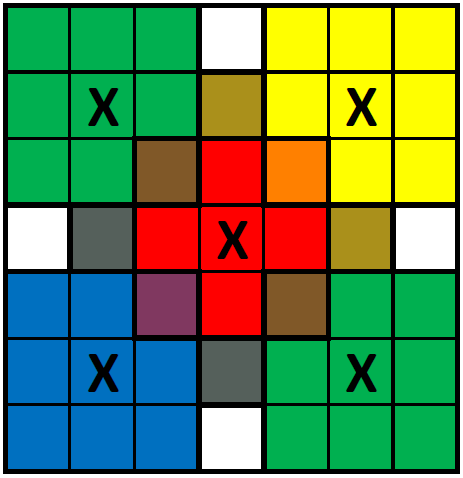
\includegraphics[width=0.5\linewidth]{images/corolle_placement}
			\end{center}
			\caption{Placement de 5 corolles sur un plateau de taille 7 (ouvertures)}\label{fig:corolle_placement}
		\end{figure}
		
		Lorsque plusieurs corolles se superposent (les zones foncées), il y à une très forte contrainte à cet endroit, car la pièce qui s'y trouve doit être possible dans toutes ces corolles.
	\end{exmp}
	
	\begin{rem}
		Actuellement, il est plus bénéfique de placer moins de corolles sur le plateau pour laisser place aux fermetures.	
	\end{rem}
\newpage	

	\subsection{Fermetures}
	
		Pour les fermetures, le principe est le même que pour les ouvertures, mais le but est différent : le but est de déterminer facilement si la résolution actuelle est viable. Par conséquent, il faut limiter au plus le nombre de fermetures. afin de déterminer la réalisation du problème le plus rapidement possible.
		
		Par conséquent, le placement des corolles se fait sur les coins (car il n'y à que 4 pièces qui peuvent y être placés)
		
		\begin{figure}[H]
			\centering
			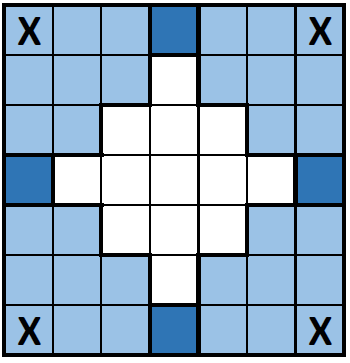
\includegraphics[width=0.5\linewidth]{images/corolle_placement_fermetures}
			\caption{Placement des corolles sur un plateau de taille 7 (fermetures)}
			\label{fig:corolle_placement_fermetures}
		\end{figure}
